%%%%%%%%%%%%%%%%%%%%%%%%%%%%%%%%%%%%%%%%%%%%%%%%%
	\begin{frame}
		\frametitle{}
	    \begin{center}
		{ {\Huge 第一章~~绪~论 (4课时)}}
	    \end{center}    
	\end{frame}

%%%%%%%%%%%%%%%%%%%%%%%%%%%%%%%%%%%%%%%%%%%%%%
\section{课程介绍}

\begin{frame}
\frametitle{课程介绍}
	\begin{center}
		\begin{figure}
		\begin{minipage}[t]{0.4\textwidth}
			\includegraphics[width=4.5cm]{figs/fig1-2.png}	
			%\caption{}
		\end{minipage}
		\begin{minipage}[t]{0.4\textwidth}
			\includegraphics[width=3.0cm]{figs/fig1-2-2.png}	
			%\caption{}
		\end{minipage}
		\end{figure}
	17世纪微积分出现,物理学家写方程,数学物理学家解方程,试图通过方程理解大千世界。
  	\end{center}
\end{frame}

\begin{frame}
	\frametitle{数理方程在数学中的位置}
	\begin{center}
		\begin{figure}
			\includegraphics[width=7cm]{figs/fig1-1.png}	
			%\caption{}
		\end{figure}
		{ 数学:逻辑,计算,分析,统计,结构}
	\end{center}
\end{frame}
%3%

\subsection{主要内容}

\begin{frame}
	\frametitle{教学内容}
	\begin{enumerate}
			\item 第一章 ~绪论(4学时):常微分方程及其解法、傅里叶变换
			 \vspace{0.2cm}
			 \item 第二章~ 偏微分方程(6学时):波动方程、热传导方程、拉普拉斯方程。
			 \vspace{0.2cm}
			 \item 第三章 ~薛定谔方程(6学时):无限深势阱、量子谐振子、Hermite多项式
            \vspace{0.2cm}
            \item 第四章 ~氢原子薛定谔方程(10学时):勒让德方程、拉盖尔(Laguerre)方程
            \vspace{0.2cm}
            \item 第五章~ 特殊函数及其应用(6学时):贝塞尔(Bessel)方程、Bessel函数
     \end{enumerate}	
\end{frame}

\begin{frame}
	\frametitle{}
	\begin{center}
		\begin{figure}
			\includegraphics[width=4.5cm]{figs/fig1-3-1.png}	
		\end{figure}
	\end{center}
	{数理方程大牛-拉普拉斯(法):拉普拉斯方程,天体力学,比如描述引力势能,时间1770年代(乾隆年间)}
\end{frame}

\begin{frame}
	\frametitle{}
	\begin{center}
		\begin{figure}
			\includegraphics[width=4.5cm]{figs/fig1-3-4.png}	
		\end{figure}
	\end{center}
		{泊松(法):Laplace方程原来是Poisson方程的特例,描述场(电场,引力场等等)}
\end{frame}

\begin{frame}
	\frametitle{}
	\begin{center}
		\begin{figure}
			\includegraphics[width=4.5cm]{figs/fig1-3-5.png}	
		\end{figure}
	\end{center}
		{勒让德(法):球坐标系下的拉普拉斯方程,可转化为勒让德方程。球谐函数,薛定谔方程解氢原子}
\end{frame}

\begin{frame}
	\frametitle{}
	\begin{center}
		\begin{figure}
			\includegraphics[width=4.5cm]{figs/fig1-3-2.png}	
		\end{figure}
	\end{center}
		{格林(英):Laplace方程无源场,泊松方程有源场,解是格林函数的叠加}
\end{frame}

\begin{frame}
	\frametitle{}
	\begin{center}
		\begin{figure}
			\includegraphics[width=4.5cm]{figs/fig1-3-3.png}	
		\end{figure}
	\end{center}
	{傅里叶(法国):分离变量法解波动方程,积分变换法解热传导方程,傅里叶级数和傅里叶变换}
\end{frame}

\begin{frame}
	\frametitle{}
	\begin{center}
		\begin{figure}
			\includegraphics[width=4.5cm]{figs/fig1-3-7.png}	
		\end{figure}
	\end{center}
	{达朗贝尔(法国):波动方程的通解,麦克斯韦方程、电磁波}
\end{frame}

\begin{frame}
	\frametitle{}
	\begin{center}
		\begin{figure}
			\includegraphics[width=4.5cm]{figs/fig1-3-6.png}	
		\end{figure}
	\end{center}
	{贝塞尔(德国):柱坐标系下的拉普拉斯方程,可转化为贝塞尔方程,解是一系列贝塞尔函数}
\end{frame}

\begin{frame}
	\frametitle{}
	\begin{center}
		\begin{figure}
			\includegraphics[width=4.5cm]{figs/fig1-3-8.png}	
		\end{figure}
	\end{center}
	{爱因斯坦(德国):扩散方程和热传导方程同类,原创扩散方程新解法(布朗运动),爱因斯坦方程}
\end{frame}

\begin{frame}
	\frametitle{}
	\begin{center}
		\begin{figure}
			\includegraphics[width=4.5cm]{figs/fig1-3-9.png}	
		\end{figure}
	\end{center}
	{薛定谔:1926年,薛定谔方程,解氢原子、氦原子,氢分子、... }
\end{frame}
%6
\begin{frame}
	\frametitle{教材与教参 :}
	\begin{enumerate}
		\item 教材:《工程数学讲义》 李明奇,钟尔杰,国防工业出版社, 待出版\\	\vspace{0.3cm}
     	参考资料:\\
		\item 《数学物理方程》 李明奇、田太心,电子科技大学出版社,2014
		\vspace{0.3cm}
		\item 《数学物理方法》 姚瑞正,梁家宝 ,武汉大学出版社,1992
		\vspace{0.3cm}
		\item 《数学物理方程与特殊函数》南京工学院数学教研组,人民教育出版社,1983
		\vspace{0.3cm}
		\item 《数学物理方程》孙振绮,机械工业出版社,2004
	\end{enumerate}	
\end{frame}

\subsection{成绩构成}
\begin{frame}
	\frametitle{成绩构成:}
		\begin{enumerate}
		\item 平时作业:10\%,
		\vspace{0.8cm}
		\item 课堂讨论:10\%,
		\vspace{0.8cm}
		\item 测验:~~ 10\%,
		\vspace{0.8cm}
		\item 期末考试:70\% .
		\end{enumerate}	
\end{frame}

%%%%%%%%%%%%%%%%%%%%%%%%%%%%%%%%%%%%%%%%%%%%%
\section{常微分方程}
\subsection{衰减与增长模型}
\begin{frame}
	\frametitle{微分方程及基本解法:}
    \begin{enumerate}
    \item 微分方程:含未知函数及其导数的方程 \\
    	$f\left(x,t, u, u_t,u_{tt}, \ldots u_{t \ldots t}, u_{x}, u_{xx}, \ldots, u_{x \ldots x} \right)=0$ \\
    	\vspace{0.5cm}
 		物理量(u)一般是时间和空间的函数。解微分方程就是要求出u(x,t)。根据阶分类;一阶微分方程、二阶微分方程、高阶常微分方程。
	 	根据未知函数自变量数目分类:常微分方程(单变量)、偏微分方程(多变量) 
    	\vspace{0.5cm}
    \item 基本解法:行波法、分离变量法、积分变换法、格林函数法、保角变换法、复变函数法、变分法、级数展开法         
    \end{enumerate}
\end{frame}

\begin{frame}
	\frametitle{一阶常微分方程}
	{\large 形态:$g(y)dy=f(x)dx$ }\\ \vspace{0.6cm}
	\textbf{解法:}若 $g(y)$ , $f(x)$ 连续 ,有\\	\vspace{0.3cm}
   	{\large 	$\int$ g(y) d y=$\int$ f(x) d x }\\	\vspace{0.3cm}
	若$g(y)$, $f(x)$  有原函数,通解为\\	\vspace{0.3cm}
	{\large $G(y)=F(x)+C$}\\	\vspace{0.3cm}
	定解条件确定C,得解!
\end{frame}

\begin{frame}
\frametitle{衰减与增长模型}
	\begin{block}{指数增长和衰减}
	\begin{itemize}
		\item 衰减与增长模型,自然界和人类社会客观存在。
		\item 分别采用指数衰减和指数增长描述,
		\item 速度大于零为增长模型,小于零为衰减模型。
	\end{itemize}
	\end{block}
\end{frame}

\begin{frame}
	\begin{exampleblock} {例1、	求解放射性衰减模型}
	\begin{equation*}
	\frac{du}{dt}	= - ru, ~~~~ u(t_0) = u_0
	\end{equation*}
	\end{exampleblock} 	
	\alert{解:} 方程可分离变量:
	\begin{align*}
		\frac{du}{u} &= - rdt\\
		\ln u &=-rt+C\\
		u(t)&=C’exp(-rt)	
	\end{align*}
	令$t=0$, 有$C‘=u_0$,得定解:
	\begin{equation*}
		u(t)=u_0 exp(-rt)
	\end{equation*}
\end{frame}


\begin{frame}
\begin{block} {Remark}
	显然,当$r>0$时, 有$t \to \infty$, $u(t) \to 0$,  衰减模型中的一个重要问题是求半衰期 T\\
	\alert{解:} 
	\begin{align*}
	\frac{1}{2}u_0 &=u(T) =u_0 exp(-rT)\\
	T &=\frac{1}{r} \ln 2  \approx \frac{1}{r} \times 0.6931	
	\end{align*}
	\end{block}
\end{frame}

\begin{frame}
	\begin{exampleblock} {例2、	求人口增长的逻辑斯蒂模型}
	\begin{equation*}
		\frac{d u}{d t}=r u (1-u/K)
	\end{equation*}
	\end{exampleblock} 	
	\alert{解:} 方程可分离变量:
	\begin{align*}
		&\frac{1}{u(1-u / K)}du =r d t \\
		&\frac{u / K+(1-u / K)}{u(1-u / K)} d u =r d t	\\
		&(\frac{1}{K-u}+\frac{1}{u} ) d u =r d t \\
		&-\ln (K-u)+\ln u =r t+C \\
	\end{align*}	
\end{frame}

\begin{frame}
	\begin{align*}
		&\ln \frac{u}{K-u}  =r t+C\\
		&\frac{u}{K-u} =\exp (r t+C)\\
		&u(t)  =\frac{K}{1+\exp (-r t-C)}	\\
	\end{align*}	
	\begin{block} {问题:}
	建立并求解:冠状病毒感染人数增长模型
	\end{block}    
\end{frame}

\begin{frame}
	\frametitle{一阶齐次方程 }
	\begin{exampleblock} {例3、	求解如下一阶微分方程}
	\begin{equation*}
		\frac{d y}{d x}=f\left(\frac{y}{x}\right) 
	\end{equation*}
	\end{exampleblock} 	
	\alert{解:} 令:$\dfrac{y}{x}=u$, 有:$y=xu$ \\ 
	求微分: $ \dfrac{d y}{d x}=u+x \dfrac{d u}{d x}$,	代回方程:\\	
	 $ u+x \dfrac{d u}{d x}=f(u) , \to \dfrac{d u}{d x}=\dfrac{f(u)-u}{x}$ ,\\ \vspace{0.2cm}
	可分离变量:
	\begin{align*}
		\int \dfrac{d u}{f(u)-u}=\int \dfrac{d x}{x} 
	\end{align*}	
\end{frame}

\begin{frame}
\begin{exampleblock} {例4、	求解一阶微分方程}
	\begin{equation*}
	\left(x-y \cos \frac{y}{x}\right) d x+x \cos \frac{y}{x} d y=0
	\end{equation*}
\end{exampleblock} 	
\alert{解:} 变量代换后可分离变量,令$\frac{y}{x}=u$, 有:$y=xu$ , \\ 
		求微分:	$d y=x d u+u d x$ ~~~~, 
		代回原方程, 得:
		\begin{equation*}
			(x-u x \cos u) d x+x \cos u(u d x+x d u)=0
		\end{equation*}	
		整理, 得可分离变量方程:
		\begin{equation*}
			\cos udu=-\frac{dx}{x}
		\end{equation*}	
		两边积分
		\begin{equation*}
			\sin u=-\ln x+C, \to  \sin \frac{y}{x}=-\ln x+C
		\end{equation*}	
\end{frame}


\begin{frame}
	\frametitle{一阶非齐次方程}
	\begin{exampleblock} {例5、	求一阶变系数非齐次方程}
	\begin{equation*}
		y^{\prime}+P(x) y=Q(x)
	\end{equation*}
	\end{exampleblock} 
	\alert{解:}  常数变易法可求解,一阶齐次线性方程 :\\
		$ y^{\prime}+P(x) y=0$  \\ 
	有通解:	{\large 	$y=Ce^{-\int P(x)dx}$}\\	\vspace{0.3cm}
		令: $C=C(x)$ ,	{\large 	$ \to y=C(x)e^{-\int P(x)dx}$} \\ 
		代回原方程:
		\begin{equation*}
			C^{\prime}(x)=\frac {Q(x)} {e^{-\int P(x)dx}}
		\end{equation*}	
\end{frame}

\begin{frame}	
		两边积分
		\begin{equation*}
			C(x)=\int Q(x)e^{\int P(x)dx} dx+c 
		\end{equation*}	
		代回通解,得解:
		\begin{equation*}
			y=Ce^{-\int P(x)dx}+e^{-\int P(x)dx}\int Q(x)e^{\int P(x)dx} dx
		\end{equation*}	
\end{frame}

\begin{frame}
	\begin{exampleblock} {例6、	求一阶常系数非齐次线性方程}
	\begin{equation*}
		y^{\prime}+Py=Q(x)
	\end{equation*}
	\end{exampleblock} 
	\alert{解:} 例5方程的解中,取P(x)=P, 得解:
	\begin{equation*}
		y=Ce^{-\int Pdx}+e^{-\int Pdx}\int Q(x)e^{\int Pdx} dx
	\end{equation*}	
\end{frame}

\begin{frame}
	\begin{exampleblock} {例7、	积分因子法求一阶全微分方程}
	\begin{equation*}
	P(x,y)dx+Q(x,y)dy=0
	\end{equation*}
	\end{exampleblock} 
	\alert{解、}  存在u(x,y),使 $ du=P(x,y)dx+Q(x,y)dy $ 成立的\\
    充要条件为:{$\dfrac{\partial P }{\partial x}=\dfrac{\partial Q }{\partial y}$ }\\	
	得通解:	{  $\displaystyle { u(x,y)=\int P(x,y)dx+\int Q(x,y)dy} $}\\ 
	若不存在,可找个积分因子 $f(x,y) $ 乘以原方程 \\  \vspace{0.2cm}
	\textbf{比如:}{\large    $ydx-xdy=0$ } 不是全微分方程,\\ 
	但 $\dfrac{ydx-xdy}{y^2}=d(\dfrac{x}{y})$ 是全微分方程, 即找到积分因子{  $ \dfrac{1}{y^2}$ } !
\end{frame}

\subsection{振动模型}

\begin{frame}
	\frametitle{振动模型}
	\begin{exampleblock} {例 8、建立简谐振动微分方程并求解}	
	\begin{center}
		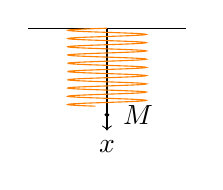
\begin{tikzpicture} [scale=0.5]
	\draw  (-2,0) -- (2,0) node[below] {};
	\draw [->] (0,0) -- (0,-2.6) node[below] {$x$};	
	\draw [orange, domain=0:-1.98, samples=200] plot({sin(\x r *30},\x);
	\draw [fill, black, circle] (0,-2.2) circle(0.3ex) node[right] {$M$};
    \end{tikzpicture} 
	\end{center}
	\end{exampleblock}
	\alert{解、} 根据牛顿第二定律,建立方程:\\
	\begin{equation*}
		F= -k x, ~~	F=Ma= M\frac{d ^2 x}{d t^2} 
	\end{equation*}
	\begin{equation*}
		\frac{d ^2 x}{d t^2} +\frac{k}{M} x =0, 
	\end{equation*}	
\end{frame}

\begin{frame}	
	得方程:
	$\displaystyle \begin{cases}
	\dfrac{d ^2 x}{d t^2} +\omega ^2 x = 0	\\
	x(t)\left |_{t=0}  =x_0  \right. , \\
	 \dfrac{dx}{dt} \left |_{t=0}  =0 \right.      	
	\end{cases}$\\
	\begin{block}{Remark}
	是常系数二阶齐次线性微分方程,通过辅助方程求解。 
	\end{block}
\end{frame}

\begin{frame}
	求解辅助方程: $u^2+\omega ^2=0$ \\
	\begin{equation*}
		u_{1, 2} =\pm i\omega     
	\end{equation*}
	方程的基本解: 
	\begin{equation*}
		x_{1} =\cos \omega t  , ~~~~	x_{2} =\sin \omega t     
	\end{equation*}
	方程通解: $x(t)=C_1 \cos \omega t +C_2 \sin \omega t $ \\  	\vspace{0.6cm}
	由初始条件得特解: $x(t)=x_0 \cos \omega t $ \\
\end{frame}

\begin{frame}
	\begin{exampleblock} {例9、	求解如下小阻尼振动微分方程:}
	\begin{equation*}
		\frac{d^2 u}{d t^2} +2\varepsilon \frac{d u}{dt} +\omega ^2 u = 0 ,  ~~~ (\varepsilon < \omega)   
	\end{equation*}
	\end{exampleblock} 
	\alert{解、} 令 $\displaystyle  u(t)= exp(-\varepsilon t) v(t) $,求微分,得:\\	
	\begin{align*}
		\frac{d u}{d t } & =exp(-\varepsilon t) [-\varepsilon v +\frac{d v}{dt}]\\
		\frac{d^2 u}{d t^2 } & =exp(-\varepsilon t) [\varepsilon ^2 v -2\varepsilon \frac{d v}{dt}+ \frac{d^2 v}{dt^2} ]
	\end{align*}
	代回原方程并整理得
	\begin{equation*}
		\frac{d^2 v}{d t^2} +(\omega ^2 - \varepsilon ^2) u = 0,  ~~~ (\varepsilon < \omega)   
	\end{equation*}
\end{frame}

\begin{frame}	
	令 $k^2 =\omega ^2 - \varepsilon ^2 $, 得简谐振动微分方程标准型。由公式 得
	\begin{equation*}
		v(t)=C_1 \cos k t +C_2 \sin k t 
	\end{equation*}
	方程的通解: 
	\begin{equation*}
		u(t)= exp(-\varepsilon t) v(t) =exp(-\varepsilon t) [ C_1 \cos k t +C_2 \sin k t] 
	\end{equation*}	
\end{frame}

\begin{frame}	
	\begin{tikzpicture}
	\datavisualization [ scientific axes,  visualize as smooth line/.list={1,2,3,4,5,6,7,8}, 
	style sheet=vary thickness , style sheet=strong colors, all axes={ticks=few}, x axis={label=$t$}, y axis={label=$u$} , style sheet=strong colors ] 
	data [format=function] {
		var set : {2};
		var x : interval [0:10] samples 200;
		func y = sin(\value x r * 10) *exp(-0.05* \value x * 10);
	}
	data [ set=lin, format=function] {
		var set : {1};
		var x : interval [0:10] samples 200;
		func y = 0;
	} ;
	\end{tikzpicture}\\
	振幅呈指数衰减.
\end{frame}

\begin{frame}
	\begin{exampleblock} {例 10、求解如下无阻尼强迫振动微分方程}
	\begin{equation*}
		\frac{d^2 u}{d t^2} + \omega ^2 u = p  \sin \omega_0 t 
	\end{equation*}
	\end{exampleblock}
	\alert{解、} 
		这是个非齐次方程,对应齐次方程的解:\\
	\begin{equation*}
		u(t)=C_1 \cos \omega t +C_2 \sin \omega t 
	\end{equation*}
	设方程的特解为:
	$ u(t) =C_0 \sin \omega_0 t $ ,
	代回原方程, 得:
	\begin{align*}
		C_0(\omega^2-\omega_{0} ^2 ) \sin(\omega_0 t)& =p\sin(\omega_0 t)\\
		C_0 & = \frac{p}{\omega^2-\omega_{0} ^2 }
	\end{align*}
	原方程的解: $ u(t)= C_1 \cos \omega t +C_2 \sin \omega t+ \frac{p}{\omega^2-\omega_{0} ^2 } \sin (\omega_0 t) $ \\
\end{frame}

\begin{frame}
	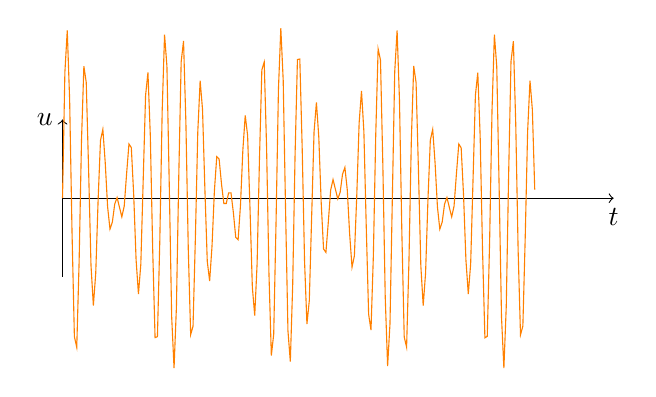
\begin{tikzpicture} 
	\centering
	% draw the axis
	\draw[->] (0,0) -- (7,0) node[below] {$t$};
	\draw[->] (0,-1) -- (0,1) node[left] {$u$};
	\draw[ orange, samples=200,domain=0:6] plot(\x, { (1-0.85^2)^(-1) * (sin( \x r *30 ) + sin (0.85*\x r *30 )      )  *0.3       } );
	\end{tikzpicture} \\
	策动频率与固有频率接近时,出现共振
\end{frame}

\begin{frame}
	\begin{block} {Remark}
	无阻尼强迫振动微分方程一般式为:
	\begin{equation*}
		\frac{d^2 u}{d t^2} + \omega ^2 u = f(t)
	\end{equation*}
	当策动函数为多项式函数,三角函数时, 待定系数法可确定特解。对于其他的情况,一般常采用常数变易法求解。
	\end{block}
\end{frame}

\subsection{常见求解方法}

\begin{frame}
\frametitle{常微分方程求解方法}
	\begin{exampleblock} {例 11、求解一阶常系数线性非齐次常微分方程}
	\begin{equation*}
		y'+py=f(x)
	\end{equation*}
	\end{exampleblock}
	\alert{解、} 对应的齐次方程是衰减数学模型,有解:\\
	\begin{center}
		$w=C_0 exp(-px)$
	\end{center} 
	应用常数变易法,设非齐次方程的解为:\\
	\begin{center}
		$y(x) =u(x) exp(-px)$
	\end{center} 
\end{frame}

\begin{frame}
	\begin{align*}
		y'&= -p u(x) exp(-px) + u'(x) exp(-px)   \\
		py&= p u(x) exp(-px)
	\end{align*}	
	代入原方程得:
	\begin{align*}
		exp(-px)u'(x)&= f(x)\\
		u(x) &= \int exp(px) f (x)dx + C
	\end{align*}
	方程的解为: $ y(x)=C exp(-px)+exp(-px) \int exp(px)f(x)dx $ \\
\end{frame}

\begin{frame}
\begin{exampleblock} {例 12、求解二阶常系数线性常微分方程}
	\begin{equation*}
		y''+py'+qy=f(x)
	\end{equation*}
	\end{exampleblock}
	\alert{解、} 对应的齐次方程为:
	\begin{equation*}
		y''+py'+qy=0
	\end{equation*}
	特征方程为:
	\begin{equation*}
		\lambda^2 +p\lambda +q=0
	\end{equation*}
	解有三种情况:
	\begin{table} [H]
	\begin{tabular}{ccc}
		两相异实根:& $\lambda_1 \ne \lambda_2 $ & \\
		两相同实根:& $\lambda_1 = \lambda_2 $  &\\
		两共轭复根:& $\lambda_1=\alpha+i\beta $, & $\lambda_2=\alpha-i\beta$\\ 
	\end{tabular}
	\end{table}
\end{frame}

\begin{frame}
	对应的齐次方程的通解:
	\begin{table} [H]
	\begin{tabular}{cccc}
		异实根:y=& $C_1 exp(\lambda_1 x)+ C_2 exp (\lambda_2 x) $  \\  
		\\
		同实根:y=&$(C_1+C_2x)  exp (\lambda_1 x) $   \\  
		\\
		共轭复根:y=& $ exp(\alpha x)  [C_1 \cos (\beta x)+ C_2 sin (\beta x)] $\\   
	\end{tabular}
	\end{table}
	根据自由项的特点,再通过待定系数法 或常数变易法求解非齐次常微分方程。
\end{frame}

\begin{frame}
\begin{exampleblock} {例 13、求二阶齐次常微分方程的通解}
	\begin{equation*}
		u''-k^2u'=0
	\end{equation*}
	\end{exampleblock}
	\alert{解、}  特征方程为:
	\begin{equation*}
		\lambda^2 -k^2=0
	\end{equation*}
	存在两相异实根: $\lambda_1=k, ~~ \lambda_2 =-k $ \\    	\vspace{0.3cm}
	通解:~~~~~~~~~u(x)= $C_1 exp(k x)+ C_2 exp (-k x) $  \\  	\vspace{0.3cm}
	写成双曲函数: u(x)= $D_1 cosh(k x)+ D_2 sinh (k x) $  \\
\end{frame}

\begin{frame}
\begin{exampleblock} {例 14、求二阶常微分方程初值问题}
	$\begin{cases}
		u'' =f, (x>0)\\
		u(0)=0, u'(0)=0
	\end{cases}$
	\end{exampleblock}
	\alert{解、} 方程两边求积分
	\begin{equation*}
		u'=\int_{0}^{\xi} f(s) ds +c_1
	\end{equation*}
	\begin{equation*}
		u(x)=\int_{0}^{x}   d\xi  \int_{0}^{\xi} f(s) ds +c_1x  +c_2
	\end{equation*}
	代入零值条件,得  $c_1=0, c_2=0$, 现交换积分次序\\
	\begin{equation*}
		u(x)=\int_{0}^{x}   ds  \int_{s}^{x} f(s) d\xi = \int_{0}^{x}  (x-s)f(s) ds 
	\end{equation*}      
\end{frame}

\begin{frame}
	\begin{exampleblock} {例 15、求二阶常微分方程的初值问题}
	$\begin{cases}
		u'' =f, (x>0)\\
		u(0)=\alpha, u'(0)=\beta
	\end{cases}$
	\end{exampleblock}
	\alert{解、}  显然,$v(x)=\alpha+\beta x$ 是如下齐次方程的解\\
		$\begin{cases}
			u'' =0, (x>0)\\
			u(0)=\alpha, u'(0)=\beta
		\end{cases}$\\
		令 $u(x)=v(x)+w(x)$, 则 w(x) 满足如下零值问题\\	
		$\begin{cases}
			u'' =f, (x>0)\\
			u(0)=0, u'(0)=0
		\end{cases}$\\	  
		由上题可写出原方程的解\\
		\begin{equation*}
			u(x)=\alpha+\beta x + \int_{0}^{x} (x-s)f(s) ds 
		\end{equation*}      
\end{frame}

\begin{frame}
	\begin{exampleblock} {例 16、常数变易法求初值问题}
	$\begin{cases}
		u'' +\omega ^2 u =f, (t>0)\\
		u(0)=0, u'(0)=0
	\end{cases}$
	\end{exampleblock}
	\alert{解、} 齐次方程有通解:
	\begin{equation*}
		u=C_1 \cos(\omega t)+C_2 \sin(\omega t)
	\end{equation*}     
	作常数变易,设非齐次方程的解可写为 
	\begin{equation*}
		u=C_1(t) \cos(\omega t)+C_2(t) \sin(\omega t)
	\end{equation*}    
\end{frame}

\begin{frame}
	求导,得
	\begin{equation*}
		u'=[C'_1(t) \cos(\omega t)+C'_2(t) \sin(\omega t)] + [  - \omega C_1(t) \sin(\omega t)+ \omega C_2(t) \cos(\omega t)  ]
	\end{equation*}    
	令 ~~ [$C'_1(t) \cos(\omega t)+C'_2(t) \sin(\omega t)$] =0,  ~~~ $\dots$  ~~~(1)\\
	\begin{equation*}
		u'= [  - \omega C_1(t) \sin(\omega t)+ \omega C_2(t) \cos(\omega t)  ]
	\end{equation*}    
	二次求导:
	\begin{equation*}
		u''= [  - \omega C'_1(t) \sin(\omega t)+ \omega C'_2(t) \cos(\omega t)  ] -\omega^2 u
	\end{equation*}  
\end{frame}

\begin{frame}
	代回原方程,得:
	\begin{equation*}
		[  - \omega C'_1(t) \sin(\omega t)+ \omega C'_2(t) \cos(\omega t)  ] =f      ~~~~  \left( 2\right)
	\end{equation*}  
	联立(1)(2), 得方程组:\\  	
	$\begin{bmatrix}
		\cos(\omega t) & \sin(\omega t) \\ 
		-\omega \sin(\omega t) & \omega\cos(\omega t)
	\end{bmatrix} $
	$\begin{bmatrix}
		C'_1(t)\\ 
		C'_2(t)
	\end{bmatrix} $ =
	$\begin{bmatrix}
		0\\ 
		f
	\end{bmatrix} $ \\ \vspace{0.3cm}
	解得:\\  
	$\displaystyle \begin{cases}
		C'_1(t)=\dfrac{1}{\omega} \sin(\omega t) f \\ 
		C'_2(t)=\dfrac{1}{\omega} \cos(\omega t) f 
	\end{cases} $ 
\end{frame}

\begin{frame}
	积分得:\\  
	$\displaystyle \begin{cases}
		C_1(t)=\dfrac{1}{\omega} [\int_{0}^{\tau} \sin(\omega \tau) f(\tau)  d\tau +c_1 ]\\ 
		C_2(t)=\dfrac{1}{\omega} [\int_{0}^{\tau} \cos(\omega \tau) f(\tau)  d\tau +c_2 ]\
	\end{cases} $ \\ \vspace{0.3cm}
	方程有解:\\
	\begin{align*}
		u=&\dfrac{1}{\omega}\cos(\omega t)[\int_{0}^{\tau} \sin(\omega \tau) f(\tau)  d\tau +c_1 ] \\
		&+\dfrac{1}{\omega} \sin(\omega t) [\int_{0}^{\tau} \cos(\omega \tau) f(\tau)  d\tau +c_2 ]
	\end{align*} \\ \vspace{0.3cm}
	代入初值条件, 得 $c_1=c_2=0$, 原方程的解:\\
	\begin{equation*}
		u=\frac{1}{\omega}\int_{0}^{\tau} \sin\omega (t-\tau)  f(\tau)  d\tau
	\end{equation*}   
\end{frame}

\begin{frame}
\frametitle{变系数二阶常微分方程}
	\begin{exampleblock} 	{例 17、求解欧拉方程}
	\begin{equation*}
		x^2 \frac{d^2 y}{d x^2} +x \frac{d y}{d x} +n^2 y =0 
	\end{equation*}     
	\end{exampleblock}	
	\alert{解、}  令 $x=exp(t) , (t=ln x)$,求微分:\\
	\begin{equation*}
		\frac{d y}{d x}  = 	\frac{d y}{d t}\frac{d t}{d x}= \frac{1}{ x}\frac{d y}{d t}  \to x \frac{d y}{d x}=	\frac{d y}{d t}
    \end{equation*} 
	\begin{equation*}
		\frac{d ^2y}{d x^2}  = 	\frac{d }{d t} ( \frac{1}{ x}\frac{d y}{d t}  )\frac{d t}{d x}=  
		\frac{1}{ x^2}(\frac{d ^2y}{d t^2} -	\frac{d y}{d t})   \to  	x^2 \frac{d^2 y}{d x^2} = \frac{d ^2y}{d t^2} -	\frac{d y}{d t}
	\end{equation*} 
	代入原方程...
\end{frame}

\begin{frame}
	方程可转化为:
	\begin{equation*}
		\frac{d^2 y}{d t^2}  +n^2 y =0 
	\end{equation*}     
	这是振动方程,有通解:$	y(t)=C_1 \cos n t +C_2 \sin n t$ \\
	代回变量,原方程的解为:
	\begin{equation*}
		y(x)=C_1 \cos (n \ln x) +C_2 \sin (n \ln x)
	\end{equation*}    
\end{frame}

\begin{frame}
	\begin{exampleblock} {例 18、求解如下形式的欧拉方程}
	\begin{equation*}
		x^2 \frac{d^2 y}{d x^2} +2x \frac{d y}{d x} -n(n+1) y =0 
	\end{equation*}     
	\end{exampleblock}
	\alert{解、} 	令 $x=exp(t) , (t=ln x) $, 代入原方程可转化为:
	\begin{equation*}
		\frac{d^2 y}{d t^2}  +\frac{dy}{dt}-n(n+1) y =0 
	\end{equation*}     
	其特征方程为
	\begin{equation*}
		\lambda^2 +\lambda -n(n+1) =0	
	\end{equation*}    
	两相异实根:
	\begin{equation*}
		\lambda_1=n, ~~~\lambda_2= -(n+1)
	\end{equation*}  
\end{frame}

\begin{frame}  
	方程的解为:
	\begin{equation*}
		y(t)=C_1 \exp (nt) +C_2 \exp (-(n+1) t)
	\end{equation*}  
	代回 t=ln x:
	\begin{equation*}
		y(x)=C_1 x^n +C_2 x^{-(n+1) }
	\end{equation*}   
\end{frame}

\begin{frame}
	\begin{exampleblock} {例 18'、求解如下形式的欧拉方程}
	\begin{equation*}
		x^2 \frac{d^2 y}{d x^2} -2x \frac{d y}{d x} +2y = \ln^2( x) -2 \ln(x) 
	\end{equation*}    
	\end{exampleblock}
	\alert{解、} 	令 $x=exp(t) , (t=ln x) $, 原方程可转化为:
	\begin{equation*}
 		\frac{d^2 y}{d t^2}  -3\frac{dy}{dt} +2 y =t^2 -2t 
 	\end{equation*}    
 	这是常系数齐次方程,其特征方程为:
 	\begin{equation*}
 		\lambda^2  -3\lambda +2  =0  \to  \lambda_1=1,   \lambda_2=2 
 	\end{equation*}   
\end{frame}


\begin{frame}
	齐次方程的通解为:
	\begin{equation*}
		y_1=C_1 e^t +C_2 e^{2t}
	\end{equation*}   
	设非齐次方程的特解为:
	\begin{equation*}
		y_2=a t^2+bt+c
	\end{equation*} 
	代回非齐次方程,得特解:
	\begin{equation*}
		y_2=\frac{1}{2} t^2+\frac{1}{2}t+\frac{1}{4}
	\end{equation*} 
	原方程的解为:
	\begin{equation*}
		y(t)=y_1+y_2=C_1 e^t +C_2 e^{2t}+\frac{1}{2} t^2+\frac{1}{2}t+\frac{1}{4}
	\end{equation*} 
\end{frame}


\begin{frame}
	代回$t=ln x $:
	\begin{equation*}
		y(x)=C_1 x +C_2 x^2+\frac{1}{2} \ln ^2 x+\frac{1}{2}\ln x+\frac{1}{4}
	\end{equation*} 
	\begin{block} {Remark}
		变量代换后,再由特征方程写通解是门艺术!
	\end{block}  
\end{frame}

\begin{frame}
	\begin{exampleblock} {例 19、幂级数方法求解 n 阶厄米方程}
	\begin{equation*}
		\frac{d^2 y}{d x^2} -2x \frac{d y}{d x} +2n y =0 
	\end{equation*}     
	\end{exampleblock}	
	\alert{解、} 	设方程有级数解
	\begin{equation*}
		y=\sum_{k=0}^{\infty} c_k x^k
	\end{equation*}     
	求导:\\
	$\begin{cases}
		y' = \sum_{k=1}^{\infty} k c_k x^{k-1} =\sum_{k=0}^{\infty} (k+1) c_{k+1} x^{k}\\
		y'' = \sum_{k=2}^{\infty} k (k-1) c_k x^{k-2} =  \sum_{k=0}^{\infty} (k+2) (k+1) c_{k+2} x^k
	\end{cases}$ \\
    代回原方程:
 \end{frame}

\begin{frame}
	\begin{equation*}
		\sum_{k=0}^{\infty} [ 2nc_k -2kc_k +(k+2)(k+1) c_{k+2}  ] x^k  =0
	\end{equation*}  
	各项系数为零,即: 
	\begin{equation*}
		2nc_k -2kc_k +(k+2)(k+1) c_{k+2} =0
	\end{equation*}   
	得系数递推式:
	\begin{equation*}
		c_{k+2} = \frac{ 2(k-n)}{(k+2)(k+1) } c_k, ~~  \left( k=0,1,2,3, ...  \right)
	\end{equation*}   
	分偶数阶和奇数阶来写,偶数阶有: \\
	$\displaystyle \begin{cases}
		c_2 =- \frac{2n}{2!} c_0\\
		c_4 = \frac{2^2n(n-2)}{4!} c_0 \\
		c_6 = -\frac{2^3n(n-2)(n-4)}{6!} c_0 \\
		c_{2m} = (-1) ^m \frac{2^mn(n-2)(n-4) ... (n-2m+2)  } {(2m)!} c_0
	\end{cases}$ \\
\end{frame}

\begin{frame}	
	同理,奇数阶有:\\
	{ $\displaystyle
		c_{2m+1} = (-1) ^m \frac{2^m (n-1) (n-3)(n-5)...(n-2m+1)  } {(2m+1)!} c_1$}\\ \vspace{0.3cm}
	所有系数求解,即幂级数求得,\\
	$\displaystyle \begin{cases}
		y_1(x)  = [1- \dfrac{2n}{2!} x^2+ \dfrac{2^2n(n-2)}{4!} x^4 -...  ] \\
		y_2(x)  = [x- \dfrac{2(n-1)}{3!} x^3+ \dfrac{2^2(n-1)(n-3) }{5!}x^5 -...  ]
	\end{cases}$ \\ \vspace{0.3cm}
	原方程的解为:
	\begin{equation*}
		y(x) =c_0y_1(x)+c_1 y_2(x).
	\end{equation*}   
\end{frame}

\section{傳里叶级数和傅里叶变换}
\subsection{傳里叶级数 }

\begin{frame}
\frametitle{傳里叶级数}
	\textbf{\large 三角式}:\\
	{\large  $\displaystyle f(x) =\dfrac{a_0}{2} +\sum_{n=1}^{\infty}  \left(  a_n \cos~ \frac{n\pi}{l} x +  b_n \sin~ \frac{n\pi}{l} x  \right) $ }\\	
	{\large $\displaystyle a_n =\frac{1}{l}  \int_{-l}^{l}  f(\xi )   \cos~ \frac{n\pi}{l} \xi d\xi  $ }\\	
	{\large $\displaystyle b_n =\frac{1}{l}  \int_{-l}^{l}  f(\xi )   \sin~ \frac{n\pi}{l} \xi d\xi   $ }\\	
\end{frame}

\begin{frame}
	\textbf{ \large 复数式:} \\  
	{\large  $\displaystyle f(x) =\sum_{n=-\infty}^{+\infty}  c_n e^{i\omega_n x} $ }\\	
	{\large $\displaystyle c_n =\frac{1}{2l}  \int_{-l}^{l}  f(\xi)    e^{-i\omega_n x}  d\xi  $ }\\	
	其中:{\large $\displaystyle   \omega_n=\frac{n\pi}{l} ,  n=...,-3,-2,-1,0,1,2,3,...   $} \\
\end{frame}

\begin{frame}
	\textbf{{\large 周期($2l$) 与 非周期 ($l~\to ~\infty $}}) \\
	{\large  $\displaystyle f(x) =\lim_{l\to \infty} \sum_{n=-\infty}^{+\infty}  c_n e^{i\omega_n x} $ }\\	
	\hspace{5em}{\large $\displaystyle =\lim_{l\to \infty} \sum_{n=-\infty}^{+\infty}  \frac{1}{2l}  [\int_{-l}^{l}  f(\xi)  e^{-i\omega_n x}  d\xi ]  e^{i\omega_n x}  $ }\\	
	\hspace{5em}{\large $\displaystyle =\frac{1}{2\pi} \int_{-\infty}^{+\infty}  [\int_{-l}^{l}  f(\xi)  e^{-i\omega x}  d\xi ]  e^{i\omega x} d\omega $ }\\
	\hspace{5em}{\large $\displaystyle =\frac{1}{2\pi} \int_{-\infty}^{+\infty}  G(\omega) e^{i\omega x} d\omega $ }\\
	\begin{block} {Remark}
		$1, \cos(x), \sin (x), \cos(2x), \sin (2x), ..., \cos(nx), \sin (nx) $, 构成正交完全集,
		$\left\{  exp(i\omega x)  \right\}$  也构成正交完全集。\\
	\end{block}
\end{frame}

\begin{frame}
%\begin{tikzpicture}
%	\draw[->] (0,0) -- (8,0) node[below] {$x$};
%	\draw[->] (0,0) -- (0,4) node[right] {$y$};
%	\draw [blue, thick, x=0.0185cm, y=2cm,
%	declare function={
%		sines(\t,\a,\b,\c,\d,\e )=1 + \a*sin(\t)+\b*sin(\t*\d)+\c*sin(\t*\e));
%	}]
%	plot [domain=0:360, samples=144, smooth] (\x,{sines(\x,0.5, 0.2, 0.1, 3, 5)}); 
%\end{tikzpicture}
	\begin{equation*}
		y=1 + 0.5\sin(x)+0.6\sin(3x)+0.7\sin(5x)
	\end{equation*}    
\end{frame}

\begin{frame}
	\begin{exampleblock} {例20、求函数的傳里叶展开式}
	$\displaystyle f(x)=\begin{cases}
		1 , ~~~ x \in [0, \pi] \\
		-1 ,~~~ x \in [-\pi, 0] \
	\end{cases}$ \\
	\end{exampleblock}
	\alert{解、} 这是个奇函数, 展开式中只有$sin$函数, 计算 $b_n$\\
	\begin{align*}
		b_n &=\frac{1}{\pi}  \int_{-\pi}^{\pi}  f(x) \sin~ \frac{n\pi}{\pi} x dx  \\	
		&=\frac{1}{\pi}  [ \int_{-\pi}^{0}  \sin n x dx - \int_{0}^{\pi}  \sin~nx dx] \\
		&=\frac{2}{\pi}  \int_{0}^{\pi}  \sin nx dx  \\
		&=\frac{2}{n\pi} [\cos nx] |_0 ^\pi =\frac{2}{n\pi} [ (-1) ^n -1]
	\end{align*}
\end{frame}

\begin{frame}
	得傳里叶展开式:
	\begin{equation*}
		f(x) = \frac{4}{\pi} \sum_{n=0}^{\infty}  \frac{1}{2k+1} \sin(2k+1) dx  
	\end{equation*}       
\end{frame}

\subsection{傳里叶变换 }

\begin{frame}
\frametitle{傳里叶变换 }
	由非周期的傳里叶级数,获得傳里叶变换公式:\\
	$\displaystyle \begin{cases}
		G(\omega) =\int_{-\infty}^{+\infty}  f(x) e^{-i\omega x} dx \\
		f(x) =\dfrac{1}{2\pi} \int_{-\infty}^{+\infty}  G(\omega) e^{i\omega x} d\omega
	\end{cases}$ \\ \vspace{0.3cm}
	{对称形式:}\\ 
	$\displaystyle \begin{cases}
		G(\omega) =\dfrac{1}{\sqrt{2\pi}} \int_{-\infty}^{+\infty}  f(x) e^{-i\omega x} dx  \equiv F[f(x)]\\
		f(x) =\dfrac{1}{\sqrt{2\pi}}  \int_{-\infty}^{+\infty}  G(\omega) e^{i\omega x} d\omega  \equiv F^{-1}[G(\omega)]
	\end{cases}$ \\	
\end{frame}

\begin{frame}
	\frametitle{}
	{\large   物理意义  }\\ 	\vspace{0.3cm}
	{\Large   $\displaystyle f(x) =\frac{1}{\sqrt{2\pi}}  \int_{-\infty}^{+\infty}  G(\omega) e^{i\omega x} d\omega $ }\\	\vspace{0.3cm}
    一个复杂时域信号总是由各种频域的波叠加形成!	\\ \vspace{0.3cm}
	tips: 一种数学物理方法的成功不是由于巧妙的谋略或者幸运的偶遇,而是因为他表达着物理真理的某个方面 ~~~~~~-------沙顿
\end{frame}

\begin{frame}
	\frametitle{}
	{\large   性质  }\\ 	\vspace{0.3cm}
    线性: $F[\alpha  f_1 +\beta f_2]=\alpha  F[f_1]+ \beta F[f_2]$ \\ \vspace{0.3cm}
    延迟: $F[e^{i\omega_0x} f(x)] = G(\omega-\omega_0) $ \\ \vspace{0.3cm}
    位移: $F[ f(x\pm x_0)] = e^{i\omega x_0 } F[f(x)]=e^{i\omega x_0 }G(\omega) $ \\ \vspace{0.3cm}
    相似: $F[ f(\alpha  x)] = \frac{1}{|\alpha |}G(\frac{\omega}{\alpha }) $ \\ \vspace{0.3cm}
    微分: $F[ f^{n} (x)] = (i\omega ) ^n F[f(x)]= (i\omega )^n G(\omega) $ \\ \vspace{0.3cm}
    积分: $F[ \int_{x_0}^{x}f (\xi) d\xi ] = \frac{1}{\omega}  F[f(x)]=\frac{1}{\omega} G(\omega) $ \\ \vspace{0.3cm}
\end{frame}

\begin{frame}
	\begin{exampleblock} {例 21、求动量表象波函数}
	{在量子力学中,一维体系在坐标表象中的波函数如下,求在动量表象中的波函数 $c(p)$}
		\begin{equation*}
			\Psi(x)=\frac{1}{\sqrt{2\pi \hbar}}  \int_{-\infty}^{+\infty} c(p) e^{\frac{i}{\hbar} px} dp 
		\end{equation*}   	
	\end{exampleblock}
	\alert{解、} 	把波函数改写成  \\	
	\begin{equation*}
		\Psi(x)= \frac{1}{\sqrt{2\pi }} \int_{-\infty}^{+\infty} \sqrt{\hbar} c(p) e^{i\frac{p}{\hbar} x} d(\frac{p}{\hbar})  
	\end{equation*}     
	根据对称型傅里叶变换公式,有: 
	\begin{equation*}
		\sqrt{\hbar} c(p) = \frac{1}{\sqrt{2\pi }} \int_{-\infty}^{+\infty} \Psi(x) e^{-i\frac{p}{\hbar} x} dx
	\end{equation*}   
\end{frame}

\begin{frame}
	得解:
	\begin{equation*}
		c(p) = \frac{1}{\sqrt{2\pi \hbar }} \int_{-\infty}^{+\infty} \Psi(x) e^{-\frac{i}{\hbar} px} dx
	\end{equation*}   
\end{frame}

%\subsection{作业}

\begin{frame}
\frametitle{作业 }
	1、求函数的傳里叶展开式:
	$\displaystyle f(x)=\begin{cases}
		\pi +x , ~~~ x \in [-\pi, 0] \\
		\pi -x ,~~~ x \in   [0, \pi] 
	\end{cases}$ \\
	2、分离变量法求方程\\
	\begin{equation*}
		\frac{dy}{dt}	=  r y (1-\frac{y}{K}), ~~~~ y(t_0) = y_0
	\end{equation*}
	3、	幂级数方法求解方程\\
	\begin{equation*}
		\frac{d^2 y}{d x^2} -2x \frac{d y}{d x} +2n y =0 
	\end{equation*}     
\end{frame}

\begin{frame}
	\frametitle{课外读物和思考}
	\begin{itemize}
		\item 为什么微分方程是线性方程?
		\item 什么是齐次微分方程的辅助方程 ?
		\item 微分方程的解为什么总与exp指数相关? 
		\item 为什么非齐次方程的解由齐次方程的解加特解确定?
	\end{itemize}	
\end{frame}

\begin{frame}
	\alert{说明:} 	定义微分算子 D
	\begin{equation*}
		D= \dfrac{d}{dx}
	\end{equation*}	
	定义线性算子 T
	\begin{equation*}
		T(a f(x) +b g(x) )  =a T(f(x)) +b T(g(x)) 
   \end{equation*}	
 	利用f(x) 和g(x)的Taylor 展开式,很容易证明微分算子 D是线性的。\\
	微分算子多项式$	L= c_0 + c_1D +c_2D^2 +...  $也是线性算子。\\
\end{frame}

\begin{frame}
    定义微分方程:
    \begin{equation*}
    	L(y)=f(x)
    \end{equation*}
    若{ $c_0$} 都是常数,称为常系数微分方程,否则称为变系数微分方程。 称$L(y)=0$为齐次方程, 	$L(y)=f(x)\ne0$为非齐次方程。 可以证明常系数微分方程是线性的,如果$y_1(x) ,  y_2(x) $是方程的解,则它们的线性叠加
    \begin{equation*}
    	y(x)=c_1y_1(x) +c_2y_2(x) 
    \end{equation*}	
    也是方程的解。
\end{frame}

\begin{frame}	
	微分算子 D的特征方程有解
	\begin{equation*}
		D(e^{nx})=n e^{nx}
	\end{equation*}	
	n 是特征值($\lambda=n$),$e^{nx}$ 属于 n 的特征矢。\\
	对于算子$L= c_0 + c_1D +c_2D^2 $,特征值为$\lambda=c_0 + c_1n +c_2n^2$ \\
	解辅助方程
	\begin{equation*}
		c_2n^2+c_0 + c_1n =0
	\end{equation*}	
	相当于求L算子特征值为零的特征矢,特征矢的线性叠加正是 L(y)=0 这个齐次方程的解。
\end{frame}

\begin{frame}
	对于非齐次方程,先求得齐次方程的解,再由初始条件确定一特解。相当于辅助方程
\end{frame}
